\chapter{Asymmetric Cryptography}

\begin{flushleft}

    \begin{figure}[h]
        \centering
        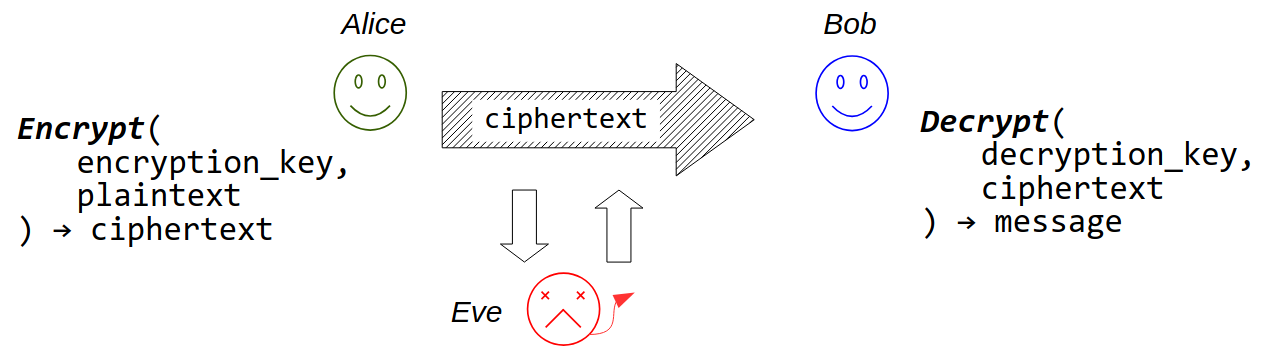
\includegraphics[width=\textwidth]{img/asym_crypto.png}
    \end{figure}

    Nella \textcolor{red}{\textbf{crittografia asimmetrica}} Alice e Bob utilizzano due chiavi differenti, infatti la \textit{encryption key} $\neq$ \textit{decryption key}, normalmente la chiave di cifrature è la pubblica e quella di decifrazione la privata. Il nome \textbf{asimmetrico} deriva dal fatto che dai requisiti per la distribuzione delle chiavi alle entità che partecipano nella comunicazione.

    \smallskip

    \textcolor{red}{\textbf{Coppia di Chiavi}}: nella crittografia asimmetrica è presente una \textbf{\textit{key pairs}} ovvero una coppia di due chiavi diverse, chiamata una \textbf{chiave secreta} (\textbf{\textit{secret key}}) e l'altra \textbf{chiave pubblica} (\textbf{\textit{public key}}). Queste due chiavi sono diverse, ma \textbf{matematicamente legate in maniera univoca}

    {\centering
        \textbf{\textit{secret key (sk)}} $\leftrightarrow$ \textbf{\textit{public key (pk)}}
    \par}

    Normalmente la \textit{secret key} è conosciuta unicamente da un'entità, mentre la \textit{public key} viene distribuita a tutti gli altri. È possibile calcolare la \textbf{pk} partendo dalla \textbf{sk}, ma non il viceversa.

    \smallskip

    Gli schemi crittografici collegati (derivati) con la crittografia simmetrica sono:
    \begin{itemize}[nosep]
        \item \textbf{\textit{digital signature}}
        \item \textbf{\textit{asymmetric encryption}} $\rightarrow$ \textbf{\textit{key encapsulation}} per \textbf{\textit{hybrid encryption}}
        \item (\textit{two party}) \textbf{\textit{key exchange (KEX)}} $\rightarrow$ \textbf{\textit{Authenticated Key Exchange}}
    \end{itemize}

    \smallskip

    \textbf{Crittografia asimmetrica} permettere di rispettare il vincolo di \textbf{confidenzialità}, permette infatti di cifrare il messaggio senza sapere la chiave segreta, ma il destinatario non ha modo di conoscere chi ha cifrato il messaggio.

    \medskip

    \textcolor{red}{\textbf{Crittografia ibrida}} \\
    L'idea è quella di incapsulare una chiave di crittografia simmetrica dentro ad un algoritmo asimmetrico:
    \begin{enumerate}[nosep]
        \item viene generata una chiave simmetrica \textbf{\textit{dek (data encryption key)}}
        \item il tutto viene incapsulato utilizzando uno schema asimmetrico attraverso l'applicazione di un \textbf{\textit{key incapsulation method (kem)}}
        \item dopo aver cifrato il messaggio con la \textbf{dek} attraverso uno schema crittografico simmetrico (ad esempio \textbf{AEAD}) viene inviato.

        \begin{figure}[h]
            \centering
            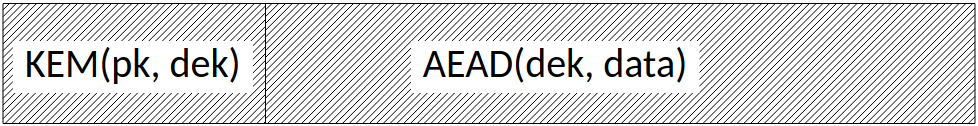
\includegraphics[width=0.75\textwidth]{img/hybrid_enc.png}
        \end{figure}
    \end{enumerate}
    La decifrazione viene applicata in maniera inversa, si decifra la \textbf{dek} con la funzione di decifrazione asimmetrica per poi decifrare il messagio con la \textbf{dek}. Può essere integrata con \textbf{firma digitale} per garantire \textbf{autenticità}.

    \medskip

    \textcolor{red}{\textbf{Firma Digitale}} \\
    In questo caso la \textbf{firma} del dato è fatta da Alice calcolando $\text{signature} = \text{sign}(\text{alice}_{sk}, \text{data})$ e viene verificata da Bob tramite $\{0, 1\} \leftarrow \text{verify}(\text{alice}_{pk}, \text{data}, \text{signature})$ in questo modo è possibile avere garanzie di \textbf{autenticità} nei settaggi asimmetrici, ma conseguentemente permette anche la garanzia su:
    \begin{itemize}[nosep]
        \item chiunque può verificare la \textit{signature} $\rightarrow$ \textbf{\textit{public verifiability}} (assumendo la correttezza della chiave pubblica).
        \item soltanto un'entità conosce il segreto: \textbf{non ripudio} (\textbf{\textit{non repudiability}}).
    \end{itemize}

    \medskip

    \textcolor{red}{\textbf{(secure) \textit{Key Exchange Protocol}}} \\
    Cercano di risolvere il \textbf{problema della distribuzioni delle chiavi} nelle configurazioni a \textbf{crittografia simmetrica}. Alice e Bob vogliono comunicare su un \textbf{canale insicuro} una chiave simmetrica condivisa senza nessuna conoscenza pregressa, per ora assumiamo che l'avversario sia \textbf{passivo}.
    
    \newpage

    \textcolor{red}{\textbf{\textit{Authenticated Key Exchange Protocol}}} \\
    Possiamo identificarla come l'unione di un \textbf{protocollo di scambio di chiavi} con la \textbf{firma digitale}, in questo caso possiamo differenziare:
    \begin{itemize}[nosep]
        \item \textbf{\textit{Server-side authenticated}}: solo il client deve verificare autenticità del server (esempio sito web).
        \item \textbf{\textit{Mutually-Authenticated}}: entrame le entità devono verificare l'autenticità dell'altra.
    \end{itemize}
    Nel caso di \textbf{\textit{Key distribution}} per \textbf{KEX} in base al \textbf{tipo} e al \textbf{contesto} di utilizzo è possibile distribuire una o entrambe le chiavi pubbliche che possono essere \textbf{permanenti} o \textbf{temporanee}.

    \begin{figure}[h]
        \centering
        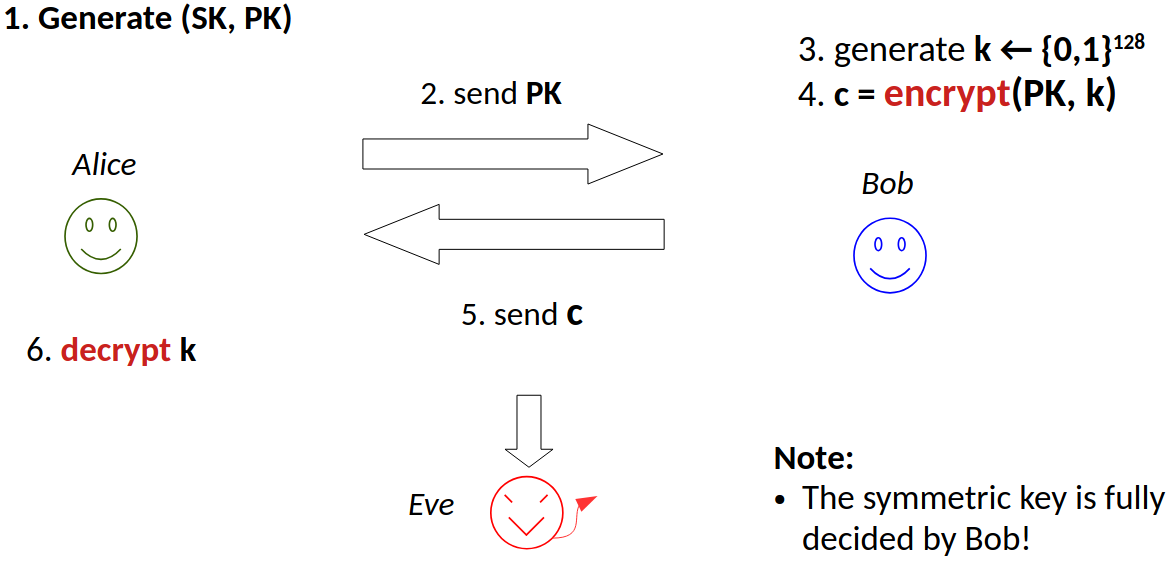
\includegraphics[width=0.75\textwidth]{img/kex.png}
        \caption{Possibile scambio di chiavi via crittografia asimmetrica}
        \label{fig:kex}
    \end{figure}

    In Fig. \ref{fig:kex} la \textit{encrypt} e la \textit{decrypt} sono riferiti allo schema asimmetrico di crittografia. In questi contesti possono comunque esserci dei problemi legati all'\textbf{autenticità della distribuzione} (sotto un attacco attivo, un avversario potrebbe distribuire chiavi false). E anche problemi legati alla \textbf{\textit{privacy}} infatti chiunque può utilizzare le nostre chiavi pubbliche (in alcuni contesti come quello della firma digitale, può essere un problema). Esistono schemi alternativi che permettono di imporre l'\textbf{anonimato}.
    
\end{flushleft}

\newpage

\section{Trapdoor One-Way Function}

\begin{flushleft}
    \textcolor{red}{\textbf{Primitive in Crittografia Simmetrica e Asimmetrica}}
    \begin{center}
        \begin{minipage}[t]{0.45\textwidth}
            \textbf{Crittografia Simmetrica}: sono basate principalmente sull'\textbf{analisi euristica}. Le funzioni sono indistinguibili da oggetti ideali come le \textbf{PRF} o \textbf{PRP}, se guardiamo il \textit{design} interno possiamo osserva la costruzione di questi blocchi su \textbf{\textit{bit-wise operation}}.
        \end{minipage}
        \hfill
        \begin{minipage}[t]{0.45\textwidth}
            \textbf{Crittografia Asimmetrica}: sono basate su - maggiormente strutturati - \textbf{problemi e algortmi matematici}. \\
            $\rightarrow$ \textbf{\textit{trapdoor one-way function}}
        \end{minipage}
    \end{center}

    Le \textbf{\textit{one-way function}} sono funzioni $f$ che sono \textbf{efficenti} da calcolare (costo polinomiale), ma che la loro funzione inversa $f^{-1}$ è \textbf{inefficente} (costo esponenziale). In crittografia simmetrica ne abbiamo già viste alcune, tra cui: le \textit{hash function} e i \textit{stream cipher} che sono \textbf{veloci}, ma completamente non strutturate e con un \textbf{comportamente impredicibile}, cosa che invece è richiesta in questo contesto. Dobbiamo ricercare tipologie di problemi matematici noti che rispecchiano queste esigenze, in modo da conoscerne il comportamento e poterlo sfruttare, ricercando quei problemi che hanno un \textbf{costo algoritmico} non trascurabile.
    \begin{itemize}[nosep]
        \item \textbf{Logaritmo discreto} (Logaritmo nei gruppi ciclici di ordine un primo): che possono basarsi su un \textbf{\textit{finite field (ff)}} costruito su un \textbf{primo intero} oppure su gruppi costruiti su \textbf{curve ellittiche}
        % campo non mi sembra corretto -> anello
        \item \textbf{rsa}: \textit{Rivest-Shamir-Adleman} che basano il problema su un \textbf{campi} di ordine \textbf{composti}, dove i fattori sono due primi di grandi dimensioni.
    \end{itemize}

    \begin{figure}[h]
        \centering
        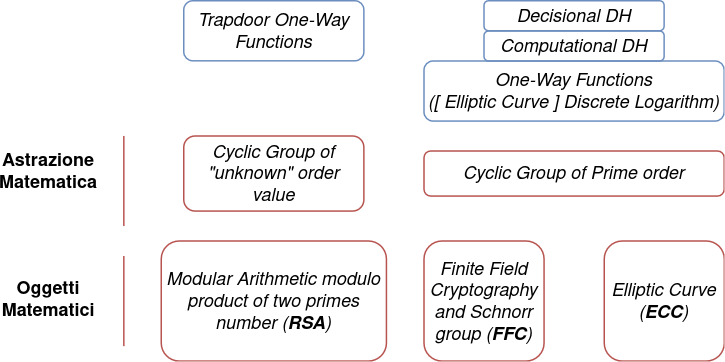
\includegraphics[width=0.75\textwidth]{img/md_crypto.png}
    \end{figure}

    Sia \textbf{RSA} che il \textbf{problema del logaritmo discreto} sono efficentemente invertibili con i \textbf{computer quantistici} (attraverso l'applicazione dell'algoritmo di \textbf{Shor}). Schemi di crittografia \textbf{\textit{post-quantum}} (promessi) si basano su problemi matematici legati a \textbf{\textit{Codes}} e \textbf{Reticoli} (\textbf{\textit{Lattices}}).
\end{flushleft}

\section{Diffie Hellman Conjectures}

\begin{flushleft}
    Consideriamo il \textbf{gruppo ciclico moltiplicativo} $\mathbb{Z}_{11}^{\times} = \{0, 1, 2, 3, 4, 5, 6, 7, 8, 9, 10\}$ e consideriamo gli elementi $2$, $3$ e $10$ andando a calcolarci il \textbf{sottogruppo ciclico} generato da questi elementi:
    \begin{itemize}[nosep]
        \item il generatore $2$ permette di ottenere il sottogruppo $\{1, 2, 3, 4, 5, 6, 7, 8, 9, 10\} \subseteq \mathbb{Z}_{11}^{\times}$
        \item il generatore $3$ permette di ottenere il sottogruppo $\{1, 3, 4, 5, 9\} \subset \mathbb{Z}_{11}^{\times}$
        \item il generatore $10$ permette di ottenere il sottogruppo $\{1, 10\} \subset \mathbb{Z}_{11}^{\times}$
    \end{itemize}
    Diremo che l'\textbf{l'ordine} del sottogruppo ottenuto dal generatore $3$ è \textbf{5} e viene definito come \textbf{\textit{Schnorr group}}. Dato un $p$ primo scrivibile come $p = 2 \cdot q + 1$ con $q$ primo, $p$ viene definito \textbf{\textit{safe prime}} (o \textbf{\textit{strong prime}}), con $p$ che sono definiti in questo modo possiamo generare 3 sottogruppi di ordine differente, rispettivamente di ordine $2$, $q$ e $2q$ (ovvero $p-1$). \\
    In algoritmi crittografici le cui primitive si basano su gruppi di ordine $p$ una scelta sbagliata del \textbf{generatore} può causare \textbf{problemi di sicurezza}.

    \smallskip

    La funzione \textbf{\textit{one-way}} che possiamo descrivere è quella del \textbf{logaritmo discreto} su un \textbf{gruppo ciclico di ordine primo}, consideriamo un generatore $g$ di un gruppo ciclico di ordine $p$ e consideriamo un $g^a \; \text{con} \; a \in \mathbb{Z}_p^{\times}$ sarà computazionalmente oneroso calcolarsi il valore $a$.

    \begin{itemize}[nosep]
        \item problema del \textbf{logaritmo discreto}: noto $g^a$ sarà difficilemnte calcolabile $a$.
        \item \textbf{\textit{computational Diffie-Hellman}} dati $g^a$ e $g^b$ sarà oneroso calcolarsi $g^{ab}$.
        \item \textbf{\textit{decisional Diffie-Hellman}} dati $g^a$ e $g^b$ sarà computazionalmente difficile distinguere $g^{ab}$ da $g^r$ dove il valore $r$ è random.
    \end{itemize}

    \newpage

    \textcolor{red}{\textbf{Curve Ellittiche}}
    \begin{itemize}[nosep]
        \item \textbf{forma di Weistrass}: $y^2 = x^3 + ax + b$
        \item \textbf{Curve Ellittiche di Edwards}:
        \begin{math}
            \begin{cases}
                x^2 + y^2 = a^2 + a^2x^2y^2 \\
                x^2 + y^2 = 1 + dx^2y^2
            \end{cases}
        \end{math}
    \end{itemize}

    \medskip

    Anche nel caso dell'applicazione di forme geometriche come le curve ellittiche, bisogna sempre ricordarsi che noi lavoreremo con numeri interi modulari.

    \medskip

    \begin{figure}[h]
        \centering
        \begin{minipage}[t]{0.45\textwidth}
            \centering
            Forma di Weistrass nell'insieme $\mathbb{R}$ \\
            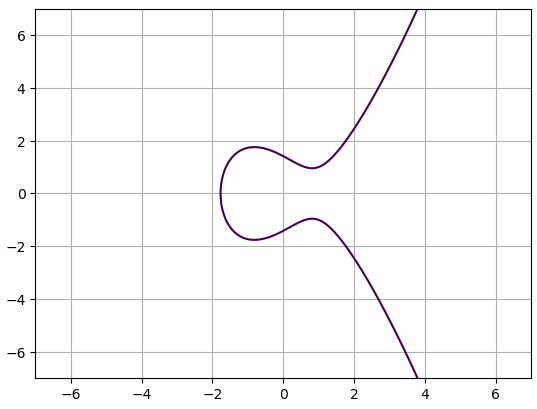
\includegraphics[width=\textwidth]{img/ec_wform.png}
            \caption{$y^2 = x^3 - 2x + 2$}
        \end{minipage}
        \hfill
        \begin{minipage}[t]{0.45\textwidth}
            \centering
            Forma di Weistrass nell'insieme $\mathbb{Z}_{149}$ \\
            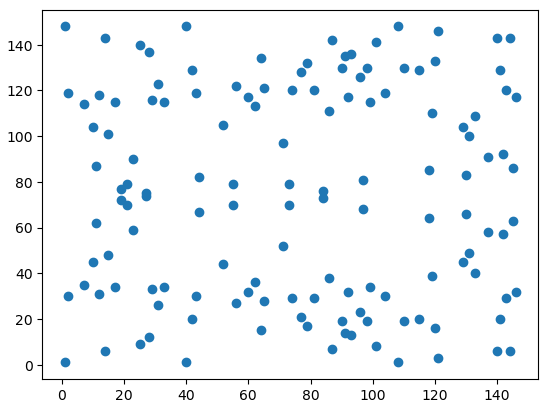
\includegraphics[width=\textwidth]{img/ec_modform.png}
            \caption{$y^2 = x^3 - 2x +2$}
        \end{minipage}
    \end{figure}

    I gruppi ciclici possono essere astratti in notazione \textbf{moltiplicativi} e \textbf{additivi}
    \begin{itemize}[nosep]
        \item \textbf{gruppi ciclici su \textit{FFC} che adottano una notazione moltiplicativa} $G_1 \cdot G_2$ è il prodotto di due interi $G_1$ e $G_2$ modulo $q$. $g^a$ con $g < q$ (intero), mentre $a < p$ (interi), le operazioni sono delle esponenziazioni modulo $q$.
        \item \textbf{gruppi ciclici su \textit{ECC} tipicamente adottano una notazione additivia} $G_1 + G_2$ è la somma di due \textbf{punti}, mentre $a \cdot G$ dove $G$ è un punto sulla curva ellittica (chiamato \textbf{\textit{base point}}), $a$ invece è uno scalare, l'operazione è quella della moltiplicazione scalare di un punto sulla curva.
        \begin{itemize}[nosep]
            \item il problema del logaritmo discreto su curve ellittiche è calcolare $a$ dato $a \cdot G$
            \item \textit{computational Diffie-Hellman} su ECC è calcolare $(a + b) \cdot G$ da $a \cdot G$ e $b \cdot G$
        \end{itemize}
    \end{itemize}
    
    \smallskip

    \textcolor{red}{\textbf{\textit{(Extra) but suggested}}} \\
    Un \textbf{punto} $P$ è formato da due coordinate $(P_x, P_y)$ ognuna delle coordinate appartiene al \textbf{campo} $\mathbb{Z}_p$ come la anche la curva. Le curve ellittiche in crittografia sono \textbf{simmetriche rispetto ad almeno un asse} (nel caso delle \textbf{curve di Edwards} ad entrambi). $-P = (P_x, -P_y)$. \\
    La rappresentazione di un punto può essere quindi \textbf{compressa} esprimendo una delle due coordinate come un bit singolo: $P = (P_x, \{0, 1\})$, infatti $P_y$ può essere ricalcolato utilizzando l'equazione della curva e il \textbf{bit} permetterà di definire il \textbf{segno}: $+ \rightarrow [0, \frac{p - 1}{2}]$ e $- \rightarrow [\frac{p - 1}{2} + 1, p - 1]$.

    \smallskip

    In certi protocolli un attaccante potrebbe fornire un \textbf{punto} $p \notin E_p(a, b)$ ovvero che le coordinate $(P_x, P_y)$ non soddisfano l'equazione della curva, oppure fornire un \textbf{punto valido} $p \in E_p(a, b)$ ma non \textbf{appartiene al gruppo crittografico} (appartiene ad un sottogruppo di ordine ``piccolo''). \\
    In entrambi gli attacchi è possibile utilizzare \textbf{proprietà matematiche} per rompere queste implementazioni incorrette, è possibile prevenirle sia a livello implementativo (aggiungendo controlli sulla validità del punto) o a livello di progettazione.

    \smallskip

    \textcolor{red}{\textbf{\textit{(extra)} Diversi Sistemi di Coordinate}} \\
    Lavorare con le \textbf{curve ellittiche} richiede molte operazioni aritmetiche sui punti. Alcuni sistemi di coordinate permettono di velocizzare i calcoli (ad esempio evitare divisioni modulari, che sono lente) a scapito di occupare più spazio in memoria (\textbf{\textit{trade-off} spazio/tempo})
    \begin{itemize}[nosep]
        \item \textbf{coordinate \textit{affine}} (``\textit{native}''): questo è il modo banale di rappresentazione $P(P_x, P_y)$, dove $P_x, P_y \in \mathbb{Z}_p$ e che soddisfano l'equazione della curva. È possibile \textbf{comprimerle} andando ad inviare una coordinata e un bit che rappresenta il segno dell'altra.
        \item \textbf{\textit{projective}} (proiettive): qui viene rappresentato ogni punto come $(X, Y, Z)$ dove $x = \frac{X}{Z}$ e $y = \frac{Y}{Z}$ in questo modo si possono eseguire operazioni tra punti senza dover fare divisioni modulo $p$, d'altro canto occupano più memoria e le formule sono più complicate.
        \item \textbf{\textit{Jacobian}} $(X, Y, Z)$ in questo caso avremo che $x = \frac{X}{Z^2}$ e $y = \frac{Y}{Z^2}$ sono ottimizzate per curve nella forma di Weistrass.
        \item \textbf{\textit{Modified Jacobian}} $(X, Y, Z, \alpha)$ come le precedenti, ma viene tenuto in memoria un valore precomputato per evitare calcoli ripetuti durante il \textbf{doubling}, vengono usate per migliorare le performance, specialmente in ambienti con risorse limitate o ottimizzazioni hardware.
    \end{itemize}

    La differenza nella rappresentazione non cambiano il punto matematico della curva. Per confrontare se due punti sono uguali, normalmente bisognerebbe tornare in coordinate affini (bisognerebbe fare la divisione, che però è molto costosa) è quindi possibile utilizzare dei ``trucchi'' algebrici per confrontare direttamente. Ad esempio in proiettivo:

    {\centering
        $X_1 \cdot Z_2 \equiv_p X_2 \cdot Z_1 \; \rightarrow \; x_1 = x_2$
    \par}

    La differente rappresentazione dei punti permette di ottimizzare le tre operazioni che normalmente vengono eseguite sulle curve ellittiche: \textbf{\textit{point addition}}, \textbf{\textit{point doubling}} e \textbf{\textit{scalar multiplication}}. In coordinate affini ogni somma di punti richiede un'inversione $\mod p$ che è ``molto lenta'' in coordinate jacobiane o proiettive ognuna di queste operazioni è effettuabile solo con somme e moltiplicazioni e quindi ``molto più veloce''.
\end{flushleft}

\section{RSA Design}

\begin{flushleft}
    Spiegazione di \textbf{\textit{Textbook RSA cryptosystem}}.

    \smallskip
    
    Nella crittografia asimmetrica abbiamo a che fare con oggetti matematici peculiari:
    \begin{itemize}[nosep]
        \item interi minori di numeri primi ($p$ in DH) o non-primi ($n$ in RSA)
        \item diverse dimensioni degli interi (ordine vs. numero di elementi di un gruppo)
        \item coordinate dei punti su una curva
        \item elementi di un gruppo che devono rientrare in sottogruppi specifici
    \end{itemize}
    
    Queste caratteristiche possono causare dei \textbf{limiti}. Pensando alla crittografia simmetrica, sappiamo che una chiave segreta deve appartenere ad un dominio binario dell'informazione con entropia uniformemente distribuita, ma nel nostro caso noi stiamo lavorando in un dominio diverso: quello dei numeri interi. Ma anche dei \textbf{richi di sicurezza}.

    \smallskip

    \textcolor{red}{\textbf{L'Insicurezza di \textit{Textbook RSA}}} \\
    Le proprietà matematiche esplicitate implicano \textbf{\textit{malleability}} (malleabilità) e \textbf{determinismo} - è possibile enumerare l'intero spazio dei messaggi, infatti la chiave di cifratura è pubblica, chiunque ci può accedere.
\end{flushleft}

\section{Diffie-Hellman Key Exchange}

\begin{flushleft}
    \begin{figure}[h]
        \centering
        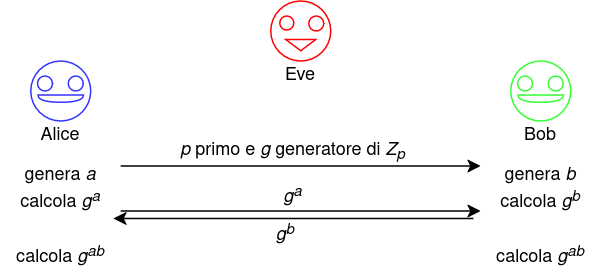
\includegraphics[width=0.55\textwidth]{img/dh.png}
    \end{figure}
    Dove $a$ e $b$ sono i \textbf{segreti temporanei} di Alice e Bob (\textbf{\textit{ephemeral keys}}), mentre $g^a$ e $g^b$ sono i \textbf{contributi pubblici} di Alice e Bob (\textbf{\textit{public contributions}}). Solo Alice e Bob possono calcolare $g^{ab}$, Eve non riesce per via del \textbf{\textit{Computational Diffie-Hellman (CDH)}} e se è valida anche la \textbf{\textit{Decisional Diffie-Hellman}} allora $g^{ab}$ è un segreto ad alta entropia che può essere utilizzato come input di una \textbf{KDF} per generare uno o più \textbf{chiavi simmetriche}. La debolezza di DH è che le parti non sono \textbf{autenticate} $\rightarrow$ \textbf{\textit{Man in the Middle Attack}}. \\
    Eve può svolgere un doppio \textbf{DH \textit{key exchange}} simultaneo con Alice e Bob interporsi nella comunicazione. \textbf{Soluzione}: \textbf{\textit{Authenticated Key Exchange}} le uniche assunzioni sono che Alice [ e Bob ] abbia una coppia di chiavi ($s_k, p_k)$ e che Bob [ Alice ] conosca la chiave pubblica.

    \smallskip

    Lo scambio di chiavi (\textbf{KEX}) può essere ricondotto a un \textbf{KEM (\textit{Key Encapsulation Mechanism})}, e applicando firme digitali a uno scambio di chiavi basato su \textbf{KEM} si ottiene un \textbf{KEX autenticato}. Con Diffie-Hellman (DH), la chiave simmetrica è contribuita da \textbf{entrambe le parti}, mentre con un KEM è decisa da una \textbf{sola parte}. A seconda del contesto, uno può essere preferito all'altro: per scopi generali, DH è la scelta tipica poiché facilita la forward secrecy grazie all'uso di chiavi ephemeral. Tuttavia, il fatto che la chiave venga decisa da un solo lato semplifica l'implementazione di alcune soluzioni di sicurezza, come la \textit{Deep Packet Inspection} su traffico cifrato (una forma di MITM legittimo). Infine, va notato che le primitive post-quantum più promettenti attualmente supportano solo scambi di chiavi basati su KEM.

\end{flushleft}

\section{Digital Signature based on DH Conjectures}

\begin{flushleft}
    \textcolor{red}{\textbf{\textit{Digital Signature Algorithm (DSA)}}}: standard alternativo alla firma di RSA. È basata sul \textbf{logaritmo discreto}, può essere implementata attraverso le curve ellittiche: \textbf{\textit{ECDSA}} (è la ragione per cui viene preferita ad RSA, scala meglio rispetto al livello di sicurezza richiesto). La via più semplice per implementare crittografia con DH è adottare un \textbf{\textit{hybrid design}}, lo standard è \textbf{\textit{Elliptic Curve Integrated Encryption Scheme (ECIES)}}.

    \begin{figure}[h]
        \centering
        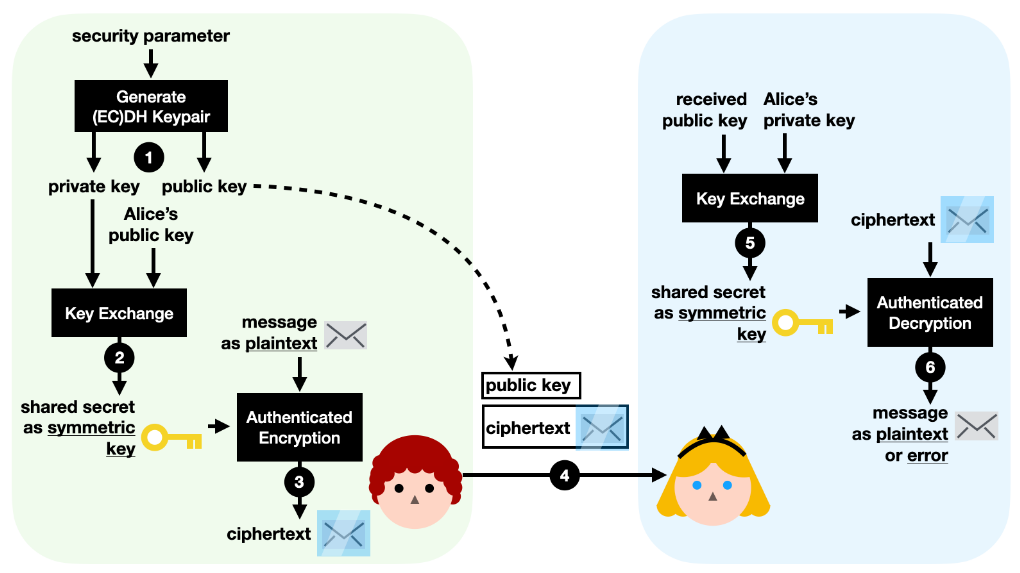
\includegraphics[width=0.85\textwidth]{img/ecies.png}
        \caption{ECIES schema}
    \end{figure}

    \medskip

    \textcolor{red}{\textbf{\textit{Digital Signature based on DH}}}: solo chi conosce il segreto può creare una firma (\textbf{\textit{signature}}) valida, ma dobbiamo distribuire una chiave pubblica che non rileva il segreto e permette di verificare la firma (\textbf{\textit{verify}}). Questa tipologia di firma digitale è del tipo \textbf{\textit{Non-Interactive Zero-Knowledge Proof}} sulla conoscenza dell'esponente segreto. Per verificare la firma il \textbf{\textit{signer}} prova la conoscenza del segreto senza rivelarla ($\neq$ \textbf{commitments} - che viene utilizzato come \textit{subroutine}).

    \begin{figure}[h]
        \centering
        \begin{minipage}[t]{0.45\textwidth}
            \textbf{\textit{Non Interactive Zero Knowledge Proof - NIZKP}} \\
            \textbf{Obiettivo}: permettere ad un \textit{prover} di dimostrare ad un \textit{verifier} di conoscere un certo segreto senza rivelarlo, e senza interazione. \\
            \textbf{Casi d'uso}: firme digitali, prova di range, \textit{blockchain} (zk-SNARKS).
        \end{minipage}
        \hfill
        \begin{minipage}[t]{0.45\textwidth}
            \textbf{\textit{Key Commitment}} \\
            \textbf{Obiettivo}: permettere ad una parte di ``\textbf{impegnarsi}'' su un \textbf{valore segreto} (ad esempio una chiave) in modo che:
            \begin{itemize}[nosep]
                \item non possa essere cambiato (\textit{binding})
                \item l'altro non la può conoscere finché non gli verrà rivelata (\textit{hiding})
            \end{itemize}
            Può essere visto come una busta sigillata crittografica. \\
            \textbf{Casi d'uso}: protocolli \textbf{KEX} per evitare attacchi \textit{MitM}, protocolli di \textit{fair exchange}.
        \end{minipage}
    \end{figure}

    \smallskip

    \textcolor{red}{\textbf{[1] \textit{Zero-Knowledge proof of Secret Exponent}}} dove il \textit{prover} è \textbf{onesto} \\
    
    \begin{figure}[h]
        \centering
        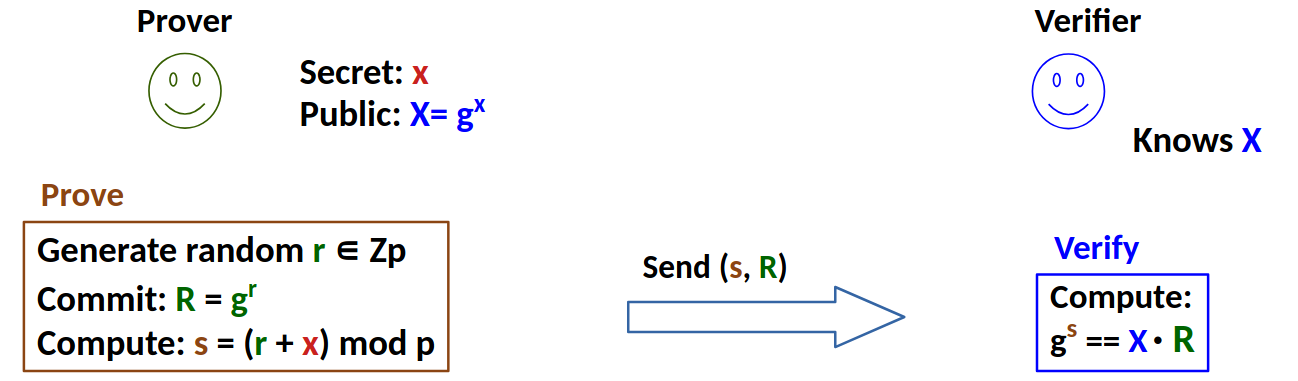
\includegraphics[width=0.95\textwidth]{img/zk_honest_prover.png}
    \end{figure}

    \begin{figure}[h]
        \centering
        \begin{minipage}[c]{0.45\textwidth}
            \textbf{Note}: osserviamo che $p$ definisce l'ordine del gruppo crittografico generato da $g$, $(r + x) \mod p$ garantisce \textbf{confidenzialità} (come un OTP), $r$ è spesso chiamato \textit{nonce} (\textbf{univocità} per la firma), ma deve essere \textbf{segreto} ed \textbf{impredicibile} $\rightarrow$ \textbf{random}, è quindi anche chiamato \textbf{\textit{one-time secret value}} della firma o \textbf{\textit{secret nonce}}.
        \end{minipage}
        \hfill
        \begin{minipage}[c]{0.45\textwidth}
            \begin{align*}
                & \textcolor{olive}{\textbf{Dimostrazione}} \quad & \\
                g^s &\equiv_p X \cdot R \\
                g^{(r + x)} &\equiv_p X \cdot R \\
                g^r \cdot g^x &\equiv_p X \cdot R \\
                R \cdot X &\equiv_p X \cdot R
            \end{align*}
        \end{minipage}
    \end{figure}

    Ma il \textit{prover} potrebbe mandare una \textbf{\textit{malicious proof}}: ovvero generare un $R$ che soddisfa la verifica in $X$ senza conoscere $x$, ad esempio: $R = g^s \cdot X^{-1}$, siccome il nostro obiettivo primario è quello di difenderci i \textit{verifier} contro \textit{prover} malevoli non possiamo adottare questo protocollo.
\end{flushleft}

\begin{boxA}

    \textcolor{orange}{\textbf{Esempio}} \\
    \textbf{Parametri pubblici}: $p = 23$, $g = 5$ e $X = 4$\\
    \textbf{\textit{Prover Malevolo}} sceglie un $s$ casuale, supponiamo $s = 7$ e calcola $R = g^s \cdot X^{-1} \mod p$ \\
    \textbf{Calcoli}: $g^s = 5^7 = 78125 \mod 23 = 18$, $X^{-1} = 4^{-1} \mod 23 = 6$ $\rightarrow$ $R = 18 \cdot 6 \mod 23 = 16$ \\
    Inviamo $(s = 7, R = 16)$ al \textit{verifier}. \\
    \textbf{Verifica}: $g^s \overset{?}{\equiv}_p X \cdot R \rightarrow 5^7 \mod 23 \overset{?}{\equiv} 4 \cdot 16 \mod 23 \rightarrow 18 \equiv 18$ \\
    La verifica va a buon fine, ma il prover non conosce $x$.
\end{boxA}

\begin{flushleft}

    \textcolor{red}{\textbf{[2] \textit{Interactive Zero-Knowledge proof}}} dove il \textit{verifier} è \textbf{onesto} \\
    \textbf{\textit{Schnorr Identification Protocol}}

    \begin{figure}[h]
        \centering
        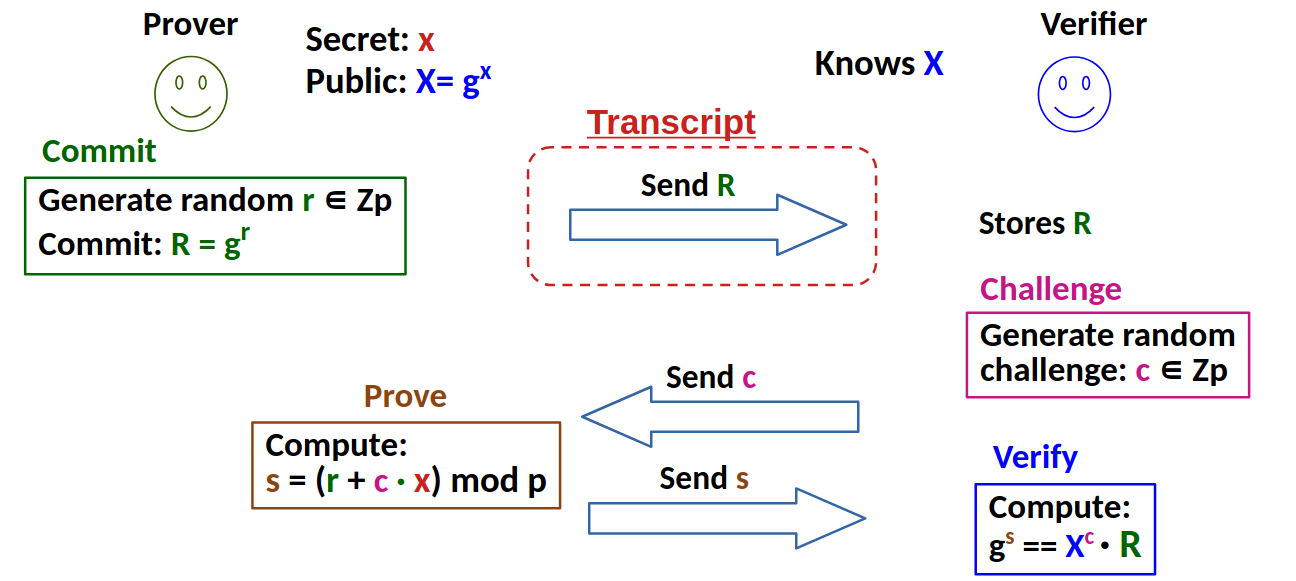
\includegraphics[width=0.95\textwidth]{img/schnorr_ip.png}
        \caption{\textit{Schnoor Signature}}
        \label{fig:schnorr_ip}
    \end{figure}

    \begin{figure}[h]
        \centering
        \begin{minipage}[c]{0.45\textwidth}
            \textbf{Note}: il \textbf{\textit{commitment}} vincola il \textit{prover} su un certo $r$ e non può cambiarlo dopo aver visto la \textit{challenge} $c$ (questo impedisce attacchi dell'\textbf{immagine iniziale}). Il \textit{verifier} sceglie la \textit{challenge} $c$ in maniera \textbf{casuale} questo impedisce al \textit{prover} di precostruire un $s$ e un $R$ in maniera malevola. Siccome $s = r + c \cdot x$ garantisce che $r$ non sia scelto a posteriori.
        \end{minipage}
        \hfill
        \begin{minipage}[c]{0.45\textwidth}
            \begin{align*}
                & \textcolor{olive}{\textbf{Dimostrazione}} \quad & \\
                g^s &\equiv_p X^c \cdot R \\
                g^{r + c \cdot x} &\equiv_p X^c \cdot R \\
                g^r \cdot g^{c \cdot x} &\equiv_p X^c \cdot R \\
                R \cdot X^c &\equiv_p X^c \cdot R
            \end{align*}
        \end{minipage}
    \end{figure}

    \medskip

    \textcolor{red}{\textbf{[3] \textit{Non-Interactive Zero-Knowledge proof of secret Exponent + Fiat-Shamir Heuristic (Transformation)}}}

    \begin{figure}[h]
        \centering
        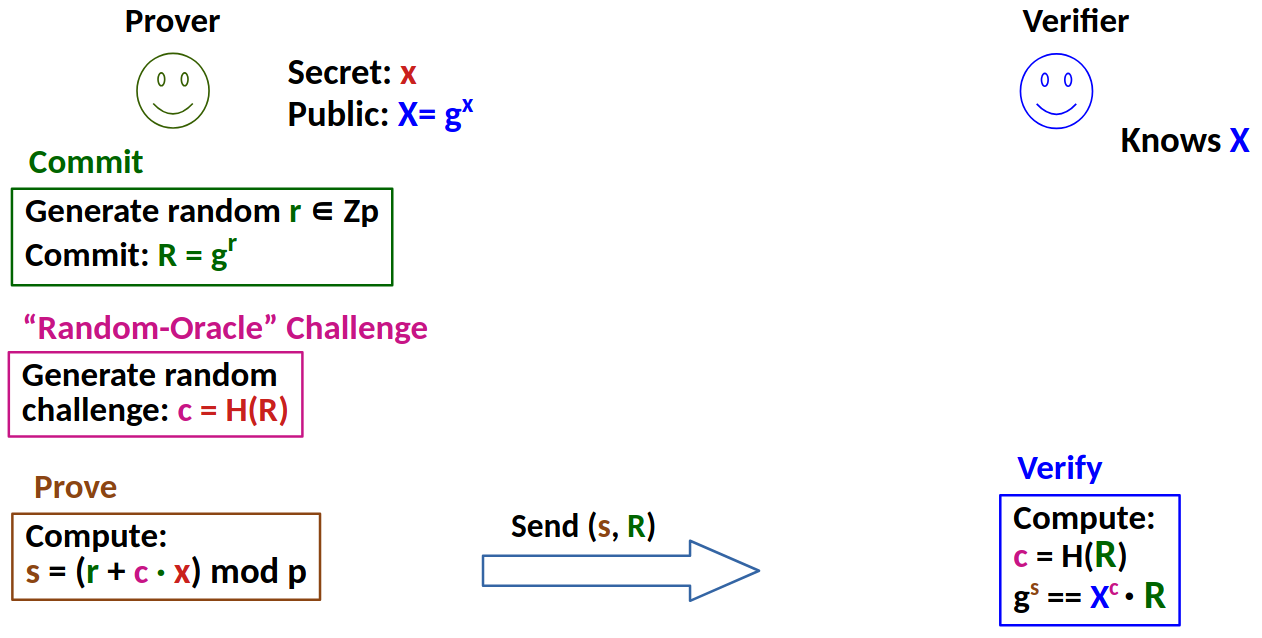
\includegraphics[width=0.95\textwidth]{img/fiat_shamir_ip.png}
        \caption{\textit{NIZKP}}
        \label{fig:fiat_shamir_ip}
    \end{figure}

    La \textit{Fiat-Shamir Heuristic} traduce qualunque \textbf{ZKP interativo} in un \textbf{NIZKP}, tuttavia aggiunge una congettura legata all'adozione di una funzione \textbf{\textit{random oracle challenge}}.
    \begin{itemize}[nosep]
        \item con \textbf{messaggi}: la \textbf{\textit{random challenge}} verrebbe calcolata $H(R \; || \; m)$ dove $m$ è il messaggio. Il \textit{prover} invierebbe al \textit{verifier} la tupla $(m, (s, R))$
        \item in alcuni casi è possibile \textbf{esplicitare la chiave pubblica} andando a calcolare la \textbf{\textit{random oracle challenge}} come $H(X \; || \; R \; || \; m)$ dove $X$ è appunta la chiave pubblica. Utili per contrastare alcuni casi di attacco in cui il \textit{verifier} venga indotto ad utilizzare un $X$ che è diverso da quello calcolato con $g^x \mod p$
    \end{itemize}

    Sono presenti anche delle varianti per quanto riguarda la \textbf{\textit{Schnorr signature}} (Fig.~\ref{fig:schnorr_ip}):

    {\centering
        \centering
        \begin{minipage}[t]{0.45\textwidth}
            \centering
            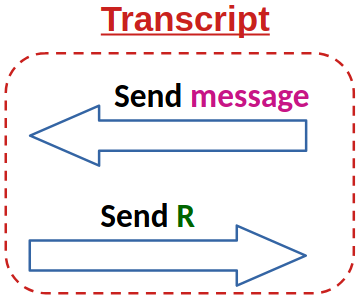
\includegraphics[width=0.55\textwidth]{img/schnorr_message_ip.png}

            \begin{flushleft}
                In questo caso il \textit{verifier} comunica un messaggio che il \textit{prover} dovrà firmare.
            \end{flushleft}

        \end{minipage}
        \hfill
        \begin{minipage}[t]{0.45\textwidth}
            \centering
            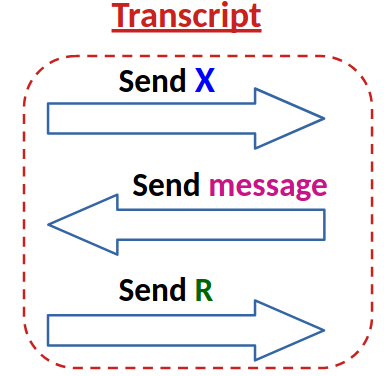
\includegraphics[width=0.55\textwidth]{img/schnorr_mX_ip.png}

            \begin{flushleft}
                In questo caso il \textit{prover} invierà prima la chiave pubblica utilizzate e successivamente il \textit{verifier} invierà il messaggio da firmare
            \end{flushleft}
        \end{minipage}
    \par}
    
    I protocolli considerati sono \textbf{probabilistici}, calcolano un random $r$ per il \textit{commitment} che - normalmente - non viene mai fornito nelle librerie. Se, però, $r$ è esposto o generato con una procedura sbagliata un avversario può ottenere la chiave segreta $x$.
    
    \smallskip

    \textcolor{red}{\textbf{\textit{Deterministic Variant}}}: generare il valore $r$ in modo \textbf{deterministico} a partire dal \textbf{messaggio} e dalla \textbf{\textit{secret key}} $x$, usando una \textbf{KDF}. Permette di evitare rischi critici dovuti alla riutilizzazione dell'$r$ e garantisce che la firma sia la stessa per uguali messaggi.
    In questo caso $r = \text{KDF}(x, m)$, la procedura per generare $r$ è \textbf{opaca} (non sa nulla) al \textit{verifier} anche perché $r$ è segreto e solamente $R$ gli viene inviato.

    \smallskip

    \textcolor{red}{\textbf{\textit{Hybrid Approaches}}} anche chiamato \textbf{\textit{hedged}} unisce la variante \textbf{deterministica} e se presente una sorgente di entropia, allora utilizza anche un valore randomico. In questo caso viene generato un $r_1 \in \mathbb{Z}_p$ e successivamente $r$ sarà calcolato come $r = \text{KDF}(x, \; \text{salt}=r_1, \; \text{info}=m)$

    \medskip

    \textcolor{red}{\textbf{\textit{EdDSA Signature (Ed22519)}}}

    \begin{figure}[h]
        \centering
        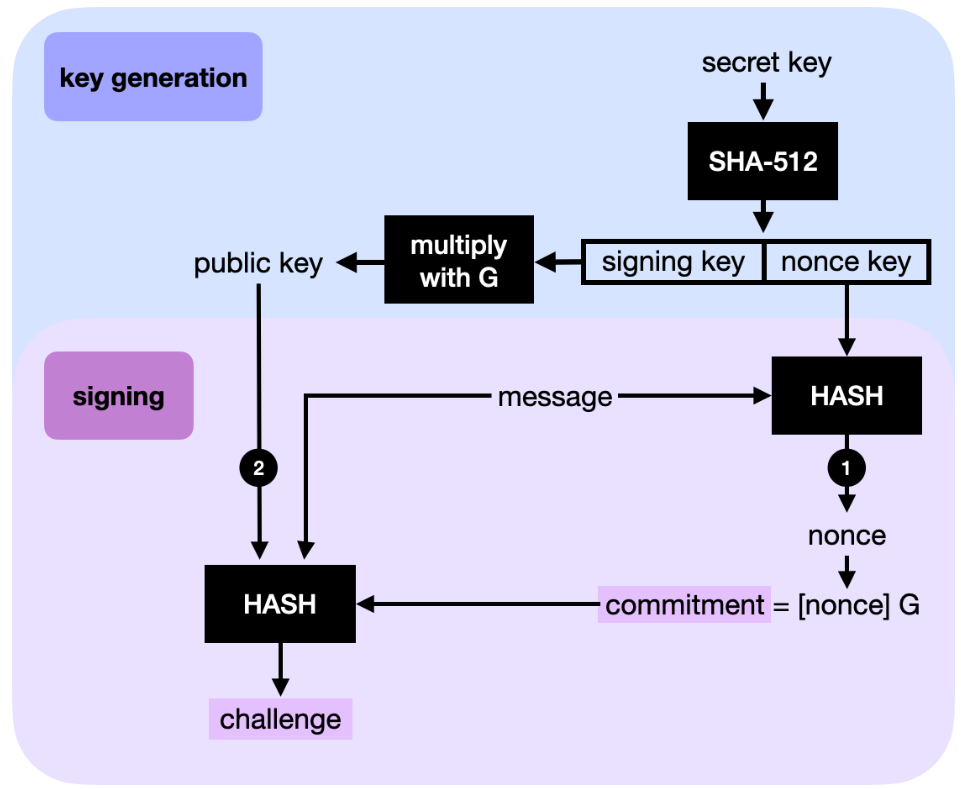
\includegraphics[width=0.75\textwidth]{img/eddsa.png}
    \end{figure}

    \textbf{SHA512} è la funzione che permette di avere chiavi \textbf{non correlate}, viene utilizzato un \textbf{HASH} per generare un ``\textbf{SIV}'' e l'altra come \textit{fiat-shamir-transformation}. \\
    Lo standard NIST per firma digitale su curve ellittiche è \textbf{ECDSA} e può essere considerata una variante della progettazione di Schnorr. \textcolor{red}{\textbf{(extra) Equazioni}}: vedi ``Algoritmi di Crittografia''.

\end{flushleft}

\begin{flushleft}
    \begin{figure}[h]
        \centering
        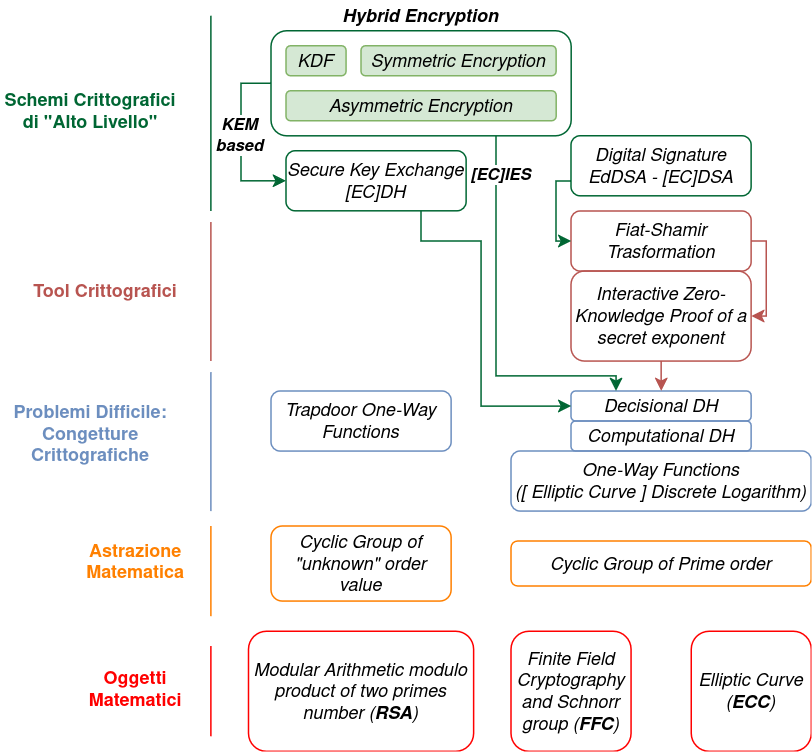
\includegraphics[width=\textwidth]{img/md_crypto_2.png}
        \caption{Mappa per gli schemi basati su \textit{[EC]DH}}
    \end{figure}
\end{flushleft}

\section{(extra) Cryptography Scheme based on RSA: PKCS\#1}
\section{(extra) "Asymmetric" Cryptography}